\documentclass[letterpaper]{article}
\usepackage{amssymb}
\usepackage{fullpage}
\usepackage{amsmath}
\usepackage{epsfig,float,alltt}
\usepackage{psfrag,xr}
\usepackage[T1]{fontenc}
\usepackage{url}


\begin{document}

\newcommand{\trace}{\mathrm{trace}}
\newcommand{\real}{\mathbb R}  % real numbers  {I\!\!R}
\newcommand{\nat}{\mathbb R}   % Natural numbers {I\!\!N}
\newcommand{\cp}{\mathbb C}    % complex numbers  {I\!\!\!\!C}
\newcommand{\ds}{\displaystyle}
\newcommand{\mf}[2]{\frac{\ds #1}{\ds #2}}
\newcommand{\book}[2]{{Luenberger, Page~#1, }{Prob.~#2}}
\newcommand{\spanof}[1]{\textrm{span} \{ #1 \}}
 \newcommand{\cov}{\mathrm{cov}}
 \newcommand{\E}{\mathcal{E}}
\parindent 0pt


\begin{center}
{\large \bf ROB 501 Exam-II (Final) Solutions}\\
20 December 2016
\end{center}

\vspace*{1cm}

%Prob. 1
\noindent \textbf{Problem 1:} The answers are (b), (c), and (d). \\

(a) False. The singular values have to satisfy $\sigma_1 \ge \sigma_2 \ge \sigma_3 \ge \sigma_4 \ge 0.$ Hence, $5\ge \sigma_3 \ge \sigma_4$, and thus $\sum_{i=1}^{4} \sigma_i \le 25.$\\

(b) True. $A>0$ implies that it is symmetric and all of its e-values are real and positive. Because $A$ is real and symmetric, there exist an orthogonal matrix $O$ and a diagonal matrix $\Lambda$ with entries equal to the e-values of $A$ such that $A O = O \Lambda$. Hence, $O \Lambda  O^\top$ is an SVD of $A$, yielding $U=V=O$.\\

(c) True. Because $\sigma_3 \ge \sigma_4 \ge 0$, $\sigma_3=0 \Rightarrow \sigma_4=0$, giving the result.\\

(d) True.  $A-B=U\left[ \begin{array}{cccc} 0 & 0 &0 &0 \\ 0 & 5 & 0 & 0\\ 0 & 0 & \sigma_3 & 0 \\ 0 & 0 & 0 & 0 \end{array} \right] V^\top$
\vspace*{1cm}

%Prob. 2
\noindent \textbf{Problem 2:} The answers are (a) (b) and (d). \\

(a) True. $\hat{x}=\alpha y_1$, where $G \alpha = c$. From the problem data, $G=<y_1,y_1> =3$ and $c=2$. Hence, $\alpha = \frac{2}{3}$.\\

(b) True. $\hat{x}=\alpha y_1$, where $G \alpha = \beta=<x_0,y_1>.$ From the problem data, $G=<y_1,y_1> =3$ and $\beta=2$. Hence, $\alpha = \frac{2}{3}$.\\

%
%
% $x_0 = x_M + x_M{^ \perp}$, with $x_M \in M$ and $x_M{^ \perp} \in M^\perp$.  Then
%$$x_M= {\rm arg}~\min_{y \in M} ||x_0-y|| ~~\text{and}~~  x_M{^ \perp} ={\rm arg}~\min_{z \in M^\perp} ||x_0-z||.$$
%From the normal equations, $x_M = \alpha_1 y^1 + \cdots + \alpha_k y^k$ when $\beta_i=<x_0,y^i>$, $1 \le i \le k$, $G \alpha = \beta$. Hence,
%$$x_M{^ \perp}=x_0 -x_M =  x_0-\left(\alpha_1 y^1 + \cdots + \alpha_k y^k\right). $$

(c) False.   We know that $M^\perp$ has dimension three. \\

(d) True. Set $A=\left[ \begin{array}{rr} a & b \\ b & d \end{array} \right]$ and compute $<A,y_1>=a$. Hence we can take $a=d=0$ and $b=1$, yielding,
$$A=\left[ \begin{array}{rr} 0 & 1 \\ 1 & 0 \end{array} \right].$$

\textbf{Remark:} As long as we set $a=0$ and $b\neq 0$, the matrix $$A=\left[ \begin{array}{rr} 0 & b \\ b & d \end{array} \right]$$
is orthogonal to $y_1$ and has rank two.


\newpage



%Prob. 3
\noindent \textbf{Problem 3:} The answers are (b) and (c). \\

(a) False. $P$ does not have to be a contraction.\\



(b) True. Because $S$ is closed and ${\cal X},$ is finite dimensional, we have that $S$ is complete.  Therefore, Cauchy sequences in $S$ have limits in $S$. \\



(c) True.  Because $P$ is a contraction mapping on $S$, $(x_k)$ is Cauchy. Because ${\cal X}$ is finite dimensional, $\bar{S}$ is complete. Hence, $(x_k)$ is a Cauchy sequence in the complete set $\bar{S}$ and thus $\exists~x^* \in \bar{S}$ such that $ x_k \to x^*$.\\



(d) False.  Let $x_0\in S$ and define for all $k\ge 1$, $x_k=x_0$. Then $\sup_{k \ge 1} ||x_k|| = ||x_0||< \infty.$ What is true? $S$ is unbounded if, and only if, there exists a sequence $(x_k)$ in $S$ such that $\sup_{k \ge 1} ||x_k|| = \infty.$\\



\vspace*{1cm}

%Prob. 4
\noindent \textbf{Problem 4:} The answers are (c) and (d). \\

The conditions to form the MVE are $E\{x\}=0$, $E\{e\}=0$, $E\{xe^\top\}=0$,  $E\{x x^\top\}=P \ge 0$, $E\{e e^\top\}=Q\ge0$ \textbf{AND} $CPC^\top + Q >0$. \\

The conditions to form BLUE are $E\{e\}=0$, \textbf{AND} $E\{e e^\top\}=Q >0$ \textbf{AND} the columns of $C$ are linearly independent.\\

MVE approaches BLUE \textbf{when} $Q>0$, the columns of $C$ are linearly independent and $P \to \infty$.\\

WLS equals BLUE \textbf{when} the columns of $C$ are linearly independent, $Q>0$, and the inner product for WLS uses the information matrix, $Q^{-1}$.\\

(a) False. See above.\\

(b) False. We need the columns of $C$ to be linearly independent which is impossible if $m<n$. \\

(c) True.  We have everything we need to form the MVE of $x$. From lecture, $ \hat{x}= \widehat{K} y$, where $$\widehat{K}=PC^\top ( C P C^\top + Q)^{-1} ~~~~\text{and}~~~~
E\{ (\hat{x}-x)(\hat{x}-x)^\top \}=P - PC^\top(CPC^\top + Q)^{-1}CP.$$
Also from lecture, the MIL gives that  $\widehat{K}=P C^\top(C PC^\top +Q)^{-1}  = (C^\top Q^{-1}C + P^{-1})^{-1} C^\top Q^{-1}$. Hence,
$$ \widehat{K} = \lim_{\rho \to \infty}  (C^\top [\rho I]^{-1}C + P^{-1})^{-1} C^\top [\rho I]^{-1}=\lim_{\rho \to \infty}  P C^\top \frac{1}{\rho}=0, $$
giving the result. \\

(d) True. Because $Q>0$, we have  $CPC^\top + Q >0$ for any $C$.\\

\newpage

%Prob. 5
\noindent \textbf{Problem 5:} The correct answer is (c). \\


(a) False. The estimated value of $x_{k+1}$, $~\hat x_{k+1} = \begin{bmatrix} 1 & 0 \\ 0 &1 \end{bmatrix} \begin{bmatrix} 5 \\ -1 \end{bmatrix} = \begin{bmatrix} 5 \\ -1 \end{bmatrix} $\\

(b) False. We have all the data to compute the Kalman gain $K_4$.
$$K_k= P_{k|k-1} C_{k}^\top (C_k P_{k|k-1} C_k^\top + Q_k)^{-1} $$
$$C_k = \begin{bmatrix} 2 \\ 2 \end{bmatrix}, ~ Q_k = 16  $$
The value we do not have in the equation is $P_{k|k-1}$, but we can compute it from $P_{k-1|k-1}$,
$$P_{k|k-1} = \begin{bmatrix} 1 & 0 \\ 0 &1 \end{bmatrix} P_{k-1|k-1} \begin{bmatrix} 1 & 0 \\ 0 &1 \end{bmatrix} + \begin{bmatrix} 1 \\ 1 \end{bmatrix} R_k \begin{bmatrix} 1 & 1 \end{bmatrix}$$
$$P_{4|3} =  \begin{bmatrix} 1 & 1 \\ 1 & 4 \end{bmatrix} + \begin{bmatrix} 9 & 9 \\ 9 &9 \end{bmatrix} = \begin{bmatrix} 10 & 10 \\ 10 & 13 \end{bmatrix}$$
We have all the values required to compute $K_4$,
$$K_4= P_{4|3} C_{4}^\top (C_4 P_{4|3} C_4^\top + Q_4)^{-1} $$



(c) True. The covariance matrix always decreases. In matrix terms, the difference is always a positive semi-definite matrix.\\

(d) False. The equality part is true, but $P_{k|k-1} - P_{k|k} \geq 0$.\\


\newpage
%Prob. 6
\noindent \textbf{Problem 6:} \\
\begin{enumerate}
 \setlength{\itemsep}{.15in}
    \renewcommand{\labelenumi}{(\alph{enumi})}
    \setlength{\itemsep}{.1in}
    \item $P=\frac{M+M^\top}{2}= \frac{1}{2}\left( \left[  \begin{array}{rrr} 4 & -1 & 6 \\ 2 & 2 &2\\0 & 0 & 9\end{array} \right] + \left[  \begin{array}{rrr} 4 & 2 & 0\\ -1 & 2 &0\\6 & 2 & 9\end{array} \right]  \right) = \left[  \begin{array}{rrr} 4 & \frac{1}{2} & 3 \\ \frac{1}{2} & 2 &1\\3 & 1 & 9\end{array} \right]$

    \item $a> 16$.

    \noindent \textbf{Solution 1} We use Schur Complements of $M=\left[  \begin{array}{ll} A & B  \\ B^\top & C \end{array} \right]$, with  $A=\left[  \begin{array}{rr} 4 & -1  \\ -1& 2 \end{array} \right]$, $B^\top=[6, ~2]$ and $C=a$. We observe $A>0$ because $4 \times 2 - (-1)\times (-1) = 7>0$. Hence,  $M>0$ if, and only if,
        $$C-B^\top A^{-1} B>0 \Leftrightarrow a - [6, ~2] \frac{1}{7} \left[  \begin{array}{rr} 2 & 1  \\ 1& 4 \end{array} \right] \left[  \begin{array}{r} 6 \\ 2 \end{array} \right] >0 \Leftrightarrow a-16>0 \Leftrightarrow a > 16$$

            \noindent \textbf{Solution 2} We use Schur Complements of $M=\left[  \begin{array}{ll} A & B  \\ B^\top & C \end{array} \right]$, with  $A=4$, $B=[-1, ~6]$ and $C=\left[  \begin{array}{rr} 2 & 2  \\ 2& a \end{array} \right]$. An easy calculations gives $C>0\Leftrightarrow 2a - 4>0$. Assuming this holds, then $M>0$ if, and only if,
        $$A-BC^{-1} B^\top>0 \Leftrightarrow a - [-1, ~6] \frac{1}{2a-4} \left[  \begin{array}{rr} 2 & -2  \\ -2& a \end{array} \right] \left[  \begin{array}{r} -1 \\ 6 \end{array} \right] >0 \Leftrightarrow 4-\frac{a+96}{2a - 4}>0 \Leftrightarrow \frac{7 a - 112}{2 a - 4}>0 \Leftrightarrow a > 16 $$
        
         \noindent \textbf{Solution 3} We use Schur Complements of $M=\left[  \begin{array}{ll} A & B  \\ B^\top & C \end{array} \right]$, with  $A=4$, $B=[-1, ~6]$ and $C=\left[  \begin{array}{rr} 2 & 2  \\ 2& a \end{array} \right]$. By inpsection, $A=4>0$. Hence,  $M>0$ if, and only if,
        $$C-B^\top A^{-1} B>0 \Leftrightarrow \left[  \begin{array}{rr} 2 & 2  \\ 2& a \end{array} \right] - \left[  \begin{array}{rr} 2 & -2  \\ -2& a \end{array} \right] \frac{1}{4} [-1, ~6] >0 \Leftrightarrow \left[  \begin{array}{rr} \frac{7}{4} & \frac{7}{2} \\ \smallskip \\\frac{7}{2}& a-9 \end{array} \right]>0 \Leftrightarrow \frac{7 a}{4}-28>0 \Leftrightarrow a > 16 $$

        \item We build $Q$ by performing Gram Schmidt on the columns of $A$ and then normalizing them to build an orthogonal matrix. Hence,
        we have $$A=[A_1 ~|~ A_2] \Leftrightarrow A_1=\left[  \begin{array}{r} 1 \\ -1\end{array} \right],~~A_2=\left[  \begin{array}{r} -1 \\ 2\end{array} \right]$$
        \begin{align*}
        v^1&= A_1=\left[  \begin{array}{r} 1 \\ -1\end{array} \right]\\
        v^2&=A_2 - \frac{<A_2,v^1>}{<v^1, v^1>}v^1 = \frac{1}{2}\left[  \begin{array}{r} 1 \\ 1\end{array} \right]
        \end{align*}
        Hence, $$Q=\left[\frac{v^1}{||v^1||}~|~ \frac{v^2}{||v^2||} \right]= \frac{1}{\sqrt{2}} \left[  \begin{array}{rr} 1 & 1  \\ -1 & 1 \end{array} \right].$$

        The matrix $R$ can be computed in several ways. The easiest here is $A= Q R \Leftrightarrow Q^\top A=R$, and thus
        $$R=\frac{1}{\sqrt{2}} \left[  \begin{array}{rr} 2 & -3  \\ 0 & 1 \end{array} \right].$$

        \newpage
        Alternatively, we use the fact that $R$ is the matrix
        representatin of $A$ in the basis $$\{  q^1:=\frac{v^1}{||v^1||}, q^2:= \frac{v^2}{||v^2|| }  \} .$$
        Therefore, we have that

\begin{align*}
A_1 &= r_{11} q^1 + r_{21}q^2 \\
&= <A_1, q^1> q^1 + <A_1, q^2> q^2\\
&= \sqrt{2} q^1 \\
\\
A_2 &= r_{12} q^1 + r_{22}q^2 \\
&= <A_2, q^1> q^1 + <A_2, q^2> q^2\\
&= -\frac{3}{2} {\sqrt{2}} q^1  + \frac{1}{2}\sqrt{2} q^2
\end{align*}

Hence $$R=\left[  \begin{array}{rr} \sqrt{2}& -\frac{3}{2} {\sqrt{2}} \\ 0 &  \frac{1}{2}\sqrt{2} \end{array} \right] = \frac{1}{\sqrt{2}} \left[  \begin{array}{rr} 2 & -3  \\ 0 & 1 \end{array} \right].$$

\end{enumerate}

\newpage


\newpage
%Prob. 7
\noindent \textbf{Problem 7:}

\noindent \textbf{Answer:}
\begin{enumerate}
	\setlength{\itemsep}{.15in}
	\renewcommand{\labelenumi}{(\alph{enumi})}
	\setlength{\itemsep}{.1in}
	\item \fbox{ \rule[-1cm]{0cm}{2cm}  $\mu_{X_1}=\begin{bmatrix} 1 \\2 \end{bmatrix}$\hskip 2cm  ~and~~ $\Sigma_{X_1}=\begin{bmatrix} 9 &2  \\2 & 4 \end{bmatrix}$\hskip 2cm }\\
	
	\item \fbox{ \rule[-1cm]{0cm}{2cm}  $\mu_{X_1|\{X_2=2\}}=\begin{bmatrix} 0.5 \\1  \end{bmatrix}$\hskip 0.8cm and~~ $\Sigma_{X_1|\{X_2=2\}} =\begin{bmatrix} 8.5 & 1 \\ 1 & 2  \end{bmatrix}$ \hskip 2cm} \\
	
	\item \fbox{ \rule[-1cm]{0cm}{2cm}  $\mu_{Z|\{Y=4\}}= 4$\hskip 4cm }
\end{enumerate}

\begin{enumerate}
    \setlength{\itemsep}{.15in}
    \renewcommand{\labelenumi}{(\alph{enumi})}
    \setlength{\itemsep}{.1in}
  \item For this part, you simply read the corresponding values of the mean and covariance from the given data. You do not have to compute anything.
  $$ \mu_{X_1}= \begin{bmatrix} 1 \\2 \end{bmatrix},~ \Sigma_{X_1}= \begin{bmatrix} 9 &2  \\2 & 4 \end{bmatrix} $$

  \item This is an immediate application of the conditioning formulas from the handout:
  $$\mu_{1|2} = \mu_1 + \Sigma_{12}\Sigma^{-1}_{22} (x_2 - \mu_2 ) $$
  $$\mu_{X_1|\{X_2=2\}} = \begin{bmatrix} 1 \\2  \end{bmatrix} + \begin{bmatrix} 1 \\2  \end{bmatrix}\times \frac{1}{2} \times (2 - 3 ) = \begin{bmatrix} 1 \\2  \end{bmatrix} + \begin{bmatrix} -0.5 \\ -1  \end{bmatrix} = \begin{bmatrix} 0.5 \\1  \end{bmatrix}$$

  $$\Sigma_{1|2} = \Sigma_{11} + \Sigma_{12}\Sigma^{-1}_{22}\Sigma_{21} $$
  $$\Sigma_{X_1|\{X_2=2\}} = \begin{bmatrix} 9 & 2 \\ 2 & 4  \end{bmatrix} -  \begin{bmatrix} 1 \\2  \end{bmatrix} \times \dfrac{1}{2} \times \begin{bmatrix} 1 & 2  \end{bmatrix} = \begin{bmatrix} 9 & 2 \\ 2 & 4  \end{bmatrix} - \begin{bmatrix} 0.5 & 1 \\ 1 & 2  \end{bmatrix} = \begin{bmatrix} 8.5 & 1 \\ 1 & 2  \end{bmatrix}$$

  \item \textbf{Solution 1:} We can first condition $Z$ and $W$ on $Y$ and then marginalize out $Z|Y$. To do this, we first re-order $\mu$ and $\Sigma$ such that $Y$ is in the top, %\textbf{Our formulas are setup for Z on the bottom}

  $$ \tilde{\mu} = \begin{bmatrix} \mu_{Y} \\ \mu_W \\ \mu_{Z} \end{bmatrix} = \begin{bmatrix} 2 \\ 1 \\ 3 \end{bmatrix}, ~ \tilde{\Sigma} = \begin{bmatrix} 4 & 2 &2  \\ 2 & 9 & 1 \\ 2 & 1 &2 \end{bmatrix}$$
 Similar to how we did earlier,
 $$\mu_{W,Z|\{Y=4\}} = \begin{bmatrix} 1 \\3  \end{bmatrix} + \begin{bmatrix} 2 \\2  \end{bmatrix}\times \frac{1}{4} \times (4 - 2 ) = \begin{bmatrix} 1 \\3  \end{bmatrix} + \begin{bmatrix} 1 \\ 1  \end{bmatrix} = \begin{bmatrix} 2 \\4  \end{bmatrix}$$
 We can pick up $\mu_{Z|\{Y=4\}}$ from this matrix and we can see $\mu_{Z|\{Y=4\}} = 4$

      \newpage

      \textbf{Solution 2:} We could first marginalize out $W$ and then condition $Z$ on $Y$ . We can see that,
       $$\mu_{Y, Z} = \begin{bmatrix} \mu_{Y} \\ \mu_{Z} \end{bmatrix} = \begin{bmatrix} 2 \\ 3 \end{bmatrix}, ~\Sigma_{Y, Z} = \begin{bmatrix} 4 & 2 \\ 2 & 2 \end{bmatrix}$$
       $$\mu_{Z|\{Y=4\}} = 3 + 2 \times \frac{1}{4} \times (4 - 2) = 3 + 1 = 4 $$
\newpage
\end{enumerate}
%Prob. 8
\noindent \textbf{Problem 8:}
\begin{enumerate}
    \setlength{\itemsep}{.15in}
    \renewcommand{\labelenumi}{(\alph{enumi})}
    \setlength{\itemsep}{.1in}
  \item \textbf{False}. The given property is \textit{uncorrelated}. If the random variables were jointly Gaussian, then uncorrelated imples independence. In general, however, as emphasized many times in lecture, the converse is false. \\

      \textbf{Grading Notes:} 1 point for the T/F answer. The rest of the points for saying ``not Gaussian'' or ``only if Gaussian'' or the equivalent. This problem was meant to be a ``freebie'' (see Google for Def.). The next two problems were not meant to be particulary easy or hard.

  \item \textbf{False}. Indeed, $\forall~n\ge 1$, $[-1,1) \subset (-1- \frac{1}{n}, 1)$. Hence, by definition of the intersection, $[-1,1) \subset \bigcap\limits_{n=1}^{\infty} (-1- \frac{1}{n}, 1)$. Moreover, $$[-1,1) = \bigcap\limits_{n=1}^{\infty} (-1- \frac{1}{n}, 1), $$
      because if $x<-1$, then there exits $1\le K<\infty$ such that $x < -1-\frac{1}{K}$, which implies that $x\not \in  (-1- \frac{1}{K}, 1)$, and thus
      $$ x \not \in \bigcap\limits_{n=1}^{\infty} (-1- \frac{1}{n}, 1). $$\\



      \textbf{Grading Notes:} 1 point for the T/F answer. After that, it depends if you computed the intersection, or if you remarked on ``infinite intersections of open sets may not be open'', etc. We'll see what the range of answers looks like and update this after the exams are graded.

  \item \textbf{False}.
  To see that $(x_n)$ itself may not converge, simply set $f\equiv0$ so that $f(x_n)=0$ converges to zero no matter what the sequence $(x_n)$ may be! Given the data, you can conclude that $\exists~x_0 \in S$ and a \underline{subsequence} $(x_{n_j})$ of $(x_n)$ such that
  $$x_{n_j} \to x_0.$$ You were not required to say anything about subsequences!
      \\

      \textbf{Grading Notes:} 1 point for the T/F answer. 2 points for noting that compactness implies the existence of a convergent subsequence, even if it is  a bit unrelated to the question. If you answered $x_n\to x_0$ and $f$ continuous implies $f(x_n) \to f(x_0)$ but the converse is false, then you received 4 points. Of course, if you gave a counterexample, as I did, then you also earned 4 points.
\end{enumerate}

\newpage
%Prob. 9
\noindent \textbf{A$^+$ Problem 9:} \fbox{$ \widehat{x}= \begin{bmatrix} \frac{1}{2}(y_1) \\  \\\frac{1}{2}(y_1)  \end{bmatrix}$}\\



 \noindent \textbf{Solution 1: (5 points)} We apply the same formulation we used for the MVE. We define our vector space as ${\cal X} := \spanof{x_1, x_2, y_1, y_2, y_2}$ with inner product given by $<z_1, z_2>:=E\{ z_1 z_2 \}$. \\

 We use the normal equations to compute for $k \in \{1,2\}$, $\widehat{x}_k = \alpha_1^k y_1+ \alpha_2^k y_2 + \alpha_2^k y_3$, where
 $$ G \alpha^k = \beta^k,~~G_{ij}=<y_i,y_j>,~~\alpha^k =\begin{bmatrix} \alpha_1^k \\ \alpha_2^k \\ \alpha_3^k\end{bmatrix},~~\beta^k =\begin{bmatrix} \beta_1^k \\ \beta_2^k \\ \beta_3^k \end{bmatrix},\text{and}~~\beta^k_j=<x_k,y_j>. $$
From the covariance matrix, we compute that
$$G=\left[  \begin{array}{ccc} 2 & 1 & 1 \\ 1 & 4 & 1 \\1 & 1 &9\end{array} \right],~~\beta^1=\begin{bmatrix} 1 \\ 0.5 \\ 0.5 \end{bmatrix}, \text{and}~~ \beta^2=\begin{bmatrix} 1 \\ 0.5 \\ 0.5 \end{bmatrix}.$$

Hence, $$\alpha^1=\alpha^2= G^{-1} \begin{bmatrix} 1 \\ 0.5 \\ 0.5 \end{bmatrix} = \begin{bmatrix} 0.5 \\ 0\\ 0 \end{bmatrix},$$
and we have that
$$\widehat{x} =  \begin{bmatrix} \frac{1}{2}y_1 \\  \\\frac{1}{2}y_1 \end{bmatrix}. $$

 \noindent \textbf{Solution 2-a: (3 points)} Solution 1 did not require the random variables to be normally distributed. For this solution and the next one, we use the fact that the variables are Gaussian. \\

Once you understand that the conditional mean is the minimum variance estimate, then this problem is an immediate application of the conditioning formula from the handout on normal random vectors when we identify
 $$X_1:=\begin{bmatrix} x_1 \\ x_2 \end{bmatrix}~~\text{and}~~X_2:=\begin{bmatrix} y_1 \\ y_2 \\ y_3\end{bmatrix}.$$

\begin{align*}
\mu_{1|2} &= \mu_1 + \Sigma_{12}\Sigma^{-1}_{22} (x_2 - \mu_2 ) \\
& =\begin{bmatrix} 0 \\ 0\end{bmatrix}  + \left[ \begin{array}{ccc} 1 & 0.5 & 0.5 \\  1 & 0.5 & 0.5\end{array} \right] \left[ \begin{array}{ccc} 2 & 1 & 1 \\1 & 4 & 1\\ 1& 1 & 9  \end{array} \right]^{-1}\big( X_2 - \begin{bmatrix} 0 \\0\\ 0 \end{bmatrix}  \big)\\
&= \left[ \begin{array}{ccc} 0.5 & 0& 0\\  0.5 & 0& 0\end{array} \right] \begin{bmatrix} y_1 \\ y_2 \\ y_3\end{bmatrix}\\
&=  \begin{bmatrix} \frac{1}{2}y_1 \\  \\\frac{1}{2}y_1 \end{bmatrix}
\end{align*}
We did invert a $3 \times 3$ matrix.



 \noindent \textbf{Solution 2-b: (5 points)} This solution is similar to \textbf{Solution 2-a}, while adding two things: (i) it shows you why $X$ only depends on $y_1$ by using the recursive form of the conditioning formula:
 $$X|_{\begin{bmatrix} Z_1 = z_1 \\ Z_2 =z_2 \end{bmatrix}} = \left( X|_{Z_2= z_2}\right)_{\left.  \right|_{\left(Z_1|_{Z_2=z_2}\right)}},$$
 and (ii), in the end, we only have to invert a $1 \times 1$ matrix.\\

We identify $Z_1=[y_2, y_3]^\top$, $Z_2=y_1$ and $X=[x_1, x_2]^\top$, and then condition on $Z_2=y_1$ to obtain
 $$\Sigma _{[X ~y_2~ y_3]^\top|_{y_1}} = \Sigma _{[X ~y_2~ y_3]^\top} - \Sigma _{[X ~y_2~ y_3]^\top {y_1}} \cdot \Sigma_{y_1, y_1}^{-1} \cdot \Sigma _{{y_1}[X ~y_2~ y_3]^\top }$$
 $$\Sigma _{[X|y)1 ~y_2|y_1~ y_3|y_1]^\top} =
 \begin{bmatrix}1 & 2 & 0.5 & 0.5\\ 2 & 6 & 0.5 & 0.5\\
 0.5 & 0.5  & 4 & 1 \\ 0.5 & 0.5 & 1 &9
 \end{bmatrix} - \begin{bmatrix} 1 \\ 1 \\ 1\\ 1 \end{bmatrix} \times  \dfrac{1}{2}\begin{bmatrix} 1 & 1 & 1& 1 \end{bmatrix} = \begin{bmatrix}0.5 & 1.5 & 0 & 0\\ 1.5 & 5.5 & 0 & 0\\
 0 & 0  & 3.5 & 0.5 \\ 0 & 0 & 0.5 & 8.5
 \end{bmatrix}$$
Due to the block of zeros in the upper-right and lower-left corners, we see that $X|y_1$ is uncorrelated to the conditional measurements $y_2|y_1, y_3|y_1$. Since we consider Gaussian variables in this case, we deduce that they are conditionally independent given $y_1$.\\

%\textbf{I think here you simply compute the conditional mean of X given y1}. That will be more clear.

 Thus we can deduce that given a set of observation MVE is dependent only on $y_1$.\\

Now to computed the conditional mean, we know that that we can ignore $y_2, y_3$.
$$\mu_{1|2} = \mu_1 + \Sigma_{12}\Sigma^{-1}_{22} (x_2 - \mu_2 ) $$

$$\mu_{X|y_1} = \begin{bmatrix} 0 \\ 0 \end{bmatrix} + \Sigma_{X,y_1}\Sigma^{-1}_{y_1,y_1} (y_1 - 0 ) $$
$$\hat X =  \begin{bmatrix} 1 \\ 1 \end{bmatrix} \times \dfrac{1}{2} \times y_1= \dfrac{1}{2}\begin{bmatrix}
y_1 \\ \\ y_1 \end{bmatrix}$$

 Note that since we take inverse of only a scalar, we are not inverting any matrix in this method,\\
 
 \noindent \textbf{The best Solution:}
\begin{figure}[h]
	\centering 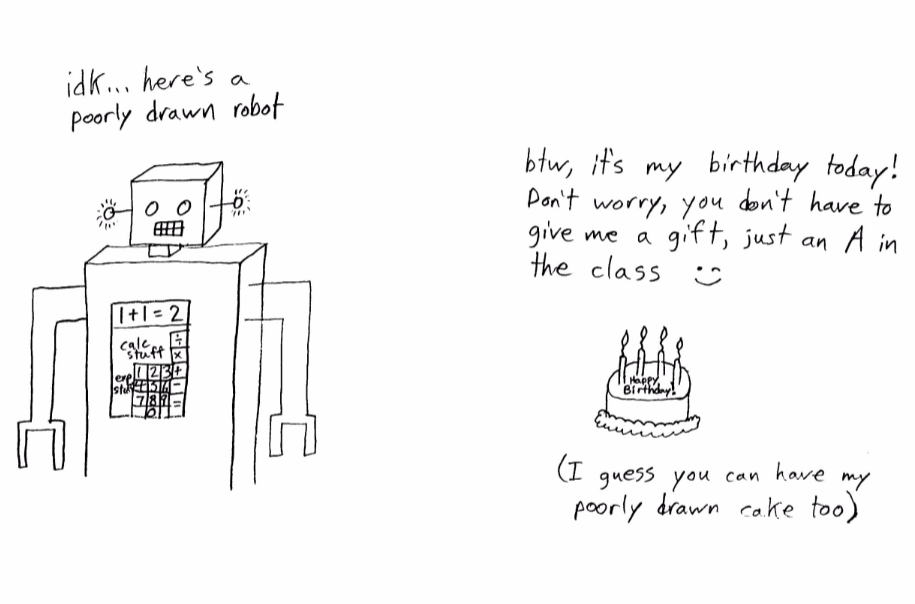
\includegraphics[width=0.55\linewidth]{ROB501_Q9.PNG}
\end{figure}
\end{document}
